\documentclass[11pt]{article}

\usepackage{amsmath}
\usepackage{graphicx}
\usepackage{fullpage}
\usepackage{placeins}
%\usepackage{amsfonts}

%\usepackage[top=1in,bottom = 1in,left = 1in,right =1in]{geometry}
%\usepackage[margin = 1in, %paperwidth=8.5in,paperheight=11in]{geometry}

\begin{document}


\title{COMP Homework}
\author{Yingjie Luan}
\maketitle

\tableofcontents

\makeatletter
\def\@seccntformat#1{%
  \expandafter\ifx\csname c@#1\endcsname\c@section
  Section \thesection:
  \else
  \csname the#1\endcsname\quad
  \fi}
\makeatother

\section{Question 1}
    \subsection{Question a}
    In solving question a, I used Matlab function called \textbf{fzero} and the \textbf{simple one dimension Newton algorithm} separately.
    
    \subsubsection{The Matlab Module}
    Here is the matlab module I used:
    \begin{verbatim}
    compressible.m:

function eval = compressible(p1)

% function [ eval ] = compressible(p1)
%
%   Indeed for solving the 1 question(a)
%
%   The reason for separating the function in 2 is due to the difficultly
%   in using function handle as a variable inside the function
%
%   Input p1 as a scalar 

d = 4.026;
eval = 433.54*520*(d^2.667)*0.7*(((p1^2-21.7^2)/(0.1894*0.7*530))^0.5)/14.7-2e6;
    \end{verbatim}
    
    \subsubsection{fzero}
    
    When using fzero, I got the solution with the value $p1=43.806$ and the function fzero is confident with its result.\\

    Below is its convergence data:
    \begin{verbatim}
    [x,f,flag]=fzero(@compressible,[25 50],optimset('Display','iter'))
 
 Func-count    x          f(x)             Procedure
    2              50        367486        initial
    3         44.6432       50497.9        interpolation
    4         43.8206       885.166        interpolation
    5          43.806       2.38209        interpolation
    6          43.806   0.000114157        interpolation
    7          43.806   4.65661e-10        interpolation
    8          43.806   4.65661e-10        interpolation
 
Zero found in the interval [25, 50]

x =

   43.8060


f =

   4.6566e-10


flag =

     1

diary off
    \end{verbatim}

\subsubsection{Newton Method}
    
    In using Newton method, I numerically calculated the differential of the given function by following the Forward Eular formula.\\
    
    Here is the codes I used:
    \begin{verbatim}
    function j_fin = fin_num_j(func,x)

% This function numerically calculate the scalar function's differential at
% the point where x = x.
%
% The input:
%   func : the function handle of the function
%   x : the value of x
%
% The output:
%   j_fin : the differential of function func at the point where x = x

h = 10*sqrt(eps);
j_fin = (feval(func,x+h)-feval(func,x))/h;

    \end{verbatim}
    
    And the answer I got by using this method is 43.806, the releated convergence data is :
    \begin{verbatim}
    mynewton(@compressible,@fin_num_j,25,1e-7,30)
   k      x_k   F(x_k)
   0       25 -1.35e+06
   1    37.73 -3.78e+05
   2    43.61 -1.18e+04
   3    43.81    -8.66
   4    43.81 -4.91e-06
   5    43.81 4.66e-10
Converged

ans =

   43.8060
\end{verbatim}

\subsubsection{The Comparsion}
\begin{enumerate}
\item Using $tic$ \& $toc$ in matlab, the time costing is as following:( Testing for 10 times, calculate the average value):
    \begin{itemize}
    \item fzero: $0.0020s$
    \item Newton Method: $0.0007057s$
    \end{itemize}
\item By reviewing the output file, we can see that newton method use \textbf 6 iterations and fzero use \textbf 8 iteration.
\item At the same time, we can see that the norm of the function at the end has been sufficiently small.(Around 1e-10)

\begin{flushleft} In summery, although this time newton method is better than fzero() but I think fzero() if well modified and the time delay just means fzero has to do all the other considerations before iteration. So I believe fzero is still better than newton method in large scale question.
\end{flushleft}


\end{enumerate}

     

    
\subsection{Question b}

In solving Question b, I used the similiar methods. We can see from the equation that the larger p1 the smaller d. From the consideration of minimizing the cost, p1 is set at $24.7$

\subsubsection{The Matlab Module}

Here is the Matlab Module:
\begin{verbatim}
function eval = compressible(d)

% function [ eval ] = compressible(p1)
%
%   Indeed for solving the 1 question(b)
%
%   The reason for separating the function in 2 is due to the difficultly
%   in using function handle as a variable inside the function
%
%   Input p1 as a scalar 

p1 = 24.7;
eval = 433.54*520*(d^2.667)*0.7*(((p1^2-21.7^2)/(0.1894*0.7*530))^0.5)/14.7-2e6;

\end{verbatim}

\subsubsection{fzero}

The final result is $d=6.2455$ and the solver is confident with its result. Belowing is the convergence data:
\begin{verbatim}
[x,f,flag]=fzero(@compressible,[4 8],optimset('Display','iter'))
 
 Func-count    x          f(x)             Procedure
    2               4  -1.39053e+06        initial
    3          5.7055       -428587        interpolation
    4         6.32373       67528.9        interpolation
    5         6.23958      -5036.72        interpolation
    6         6.24542       -52.268        interpolation
    7         6.24548    0.00073734        interpolation
    8         6.24548   -6.0536e-09        interpolation
    9         6.24548             0        interpolation
 
Zero found in the interval [4, 8]

x =

    6.2455


f =

     0


flag =

     1
\end{verbatim}

\subsubsection{Newton Method}

The solver got the result at $6.2455$\\


Belowing is the convergence data:
\begin{verbatim}
mynewton(@compressible,@fin_num_j,4,1e-7,30)
   k      x_k   F(x_k)
   0        4 -1.39e+06
   1    7.422 1.17e+06
   2    6.395 1.31e+05
   3    6.248 2.49e+03
   4    6.245    0.966
   5    6.245 1.65e-07
   6    6.245        0
Converged

ans =

    6.2455
\end{verbatim}

\subsubsection{The Comparsion}

\begin{enumerate}

\item We use the same method and after testing if for 10 times and the average value is as following:
    \begin{itemize}
    \item fzero: $0.0024s$
    \item newton: $0.0011s$
    \end{itemize}
\item By reviewing the output file, newton method used \textbf 7 iterations and fzero used \textbf 9 iterations
\item Both results satisfy the function nicely while it reduces the evaluation value down to a significantly small value.
\end{enumerate}

The summery is the same. In simple situation the newton method costs less time.


\section{Question 2}

\subsection{Question a}

\subsubsection{Exhaustive Search}
I used grid search method to solve this question. The so called grid search method is to split the range (-400,-400) to (400,400) into multiple grid and use each grid at the testing point.\\
In total, I use the interval of 10 and split it into a grid of 81*81 which will produce 6561 results in all.\\

\FloatBarrier
Figure \ref{fig:grid} is the summery that I draw to illustrate that point:\\

\begin{figure}
\centering
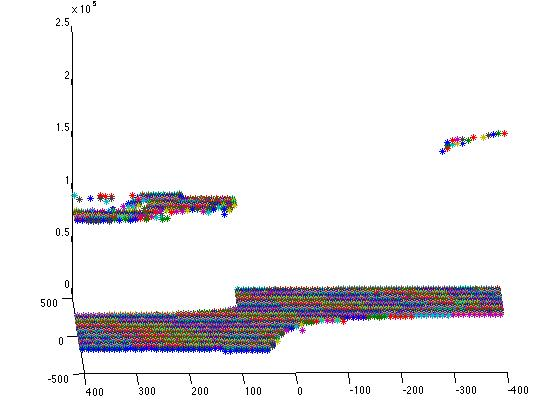
\includegraphics[scale=0.4]{p1.png}
\caption{Classified region}
\begin{minipage}{0.75\textwidth} % choose width suitably
{\footnotesize As we can see from the figure, the 3 roots have been clearly classified by their vector length value. Note from this figure we can also found out the relationship between the starting point and the root founded.(Because the convergence data means more than 6000 iteration of the fsovle I cannot include it inside this document)}
\end{minipage}
\label{fig:grid}
\end{figure}

\FloatBarrier


Here is the script for doing the exhustive search:
\begin{verbatim}
grid_search_q2a.m

%   Grid Search script: for question 2
%
%   This script will using matlab built in function fsolve to try to solve 
%   the loran.m function. 
%   The starting points are giving at the interval of 10,starting from
%   -400 to 400 along x axis and y axis
%
%   This program will produce 81*81 answers, and it will took approximatly
%   5 minuts to run through.

clear all;
[x_mesh,y_mesh] = meshgrid(-400:10:400);
flag = zeros(length(x_mesh),length(x_mesh));
answ = cell(length(x_mesh),length(x_mesh));
f = zeros(length(x_mesh),length(x_mesh));
error_rec = cell(length(x_mesh),length(x_mesh));
for x_axis = 1:length(x_mesh)
    for y_axis = 1:length(x_mesh)   
        start_p = [x_mesh(x_axis,y_axis),y_mesh(x_axis,y_axis)];
        try
        [answ_temp,f_temp,flag_temp]=fsolve(@(x)loran(x,[103.5070,226.2602,450.8810]),start_p);
        answ{x_axis,y_axis} = answ_temp;
        f(x_axis,y_axis) = f_temp;
        flag(x_axis,y_axis) = flag_temp;
        catch err
            warning('failed');
            error_rec{x_axis,y_axis} = err.identifier;
            answ{x_axis,y_axis} = nan;
            f(x_axis,y_axis) = nan;
        end           
    end
end

ind = find(flag==0);
answ(ind)={nan};
f(ind) = nan;

ind = find(flag==-2);
answ(ind)={nan};
f(ind) = nan;
\end{verbatim}
And here is the script for doing the plot:
\begin{verbatim}
answ_val_mesh.m

%   Plotting script.
%
%   This script uses the variable called answ generated by the script
%   called grid_search_q2a.m. Which is also available from the saved matlab
%   workspace called grid_search.mat
%
%   By pursumation, I think treating the space coordinator as a vector,
%   each space coordinator both will be different in x and y, and it is 
%   will very like the size of the vector which is sqrt(x^2+y^2) 
%   is also different.
%
%   The plot has successfully took the final answ into 3 aprt.

answ_val = zeros(size(answ));
size_temp = size(answ);
for t = 1:size_temp(1)*size_temp(2)
    point = answ{t};
    
    if ~isnan(point)
        val = point*point';
        answ_val(t) = val;
    else
        answ_val(t) = nan;
    end
end
        
plot3(x_mesh,y_mesh,answ_val,'*');    

temp1 = find(answ_val>1.5*10^5);
case1 = cell2mat(answ(temp1));
case1_mean = mean(case1);

temp2 = find(answ_val>7*10^4&answ_val<1.5*10^5);
case2 = cell2mat(answ(temp2));
case2_mean = mean(case2);

temp3 = find(answ_val<7*10^4);
case3 = cell2mat(answ(temp3));
case3_mean = mean(case3);
\end{verbatim}

\subsubsection{The result}
And by analyzing the result I split the region into 3 categories and calculate its average values one by one, 
which is the following:

\begin{enumerate}
\item answer1: $[-293.5926,-350,0862]$
\item answer2: $[201.0316,253.2789]$
\item answer3: $[34.1561,119.0978]$
\end{enumerate}

\subsubsection{Justifications}
The correct answer should be answer 2. I have 2 justification for that:

\begin{enumerate}

\item I draw out the situation using the function called \textit{show\_case\_q2a.m} which gives us the hints that answer2 is the right one.

\begin{figure}[h]
\centering
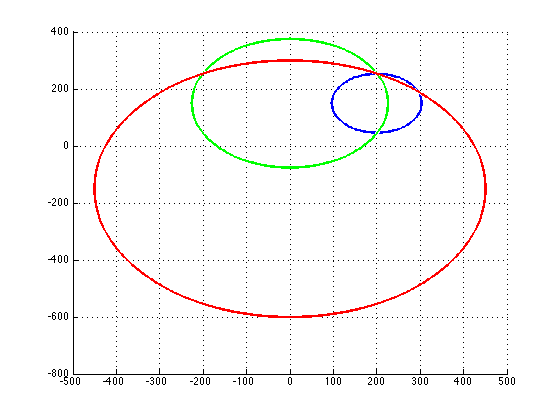
\includegraphics[scale=0.2]{p2.png}
\caption{Drawing hints}

\end{figure}

\item By calculating the distance between the answers and the observatory pairs to paris(That its norm value), we can see only answer 2 satisfy the parameter called \textit{Measured distance to object}.



\end{enumerate}

\subsection{Question b}
\subsubsection{Physical Explanation}
Due to the error within the data, we can not guarantee the correctness of the data itself. This simple method treat the error itself as a variable and successfully convert the over determining question( 2 variables and 3 functions) into a fixed answer question. The error $e$ stand for the error due to the natural characteristic of the problem itself like we cannot get a 100\% percent correct distances and we must will have some error over the recording of the data and the error within the transmitting of the data etc..

The error can be minimized by improving the quality of the data as we can see from follwing questions.

And as we can see from the formula, the meaning of error $e$ is in fact assuming that all the error was generated by $da$, and accepting the error means if we correct the data da by that error e we can get a correct answer. The following picture illustrate this point.

\begin{figure}[h]
\centering
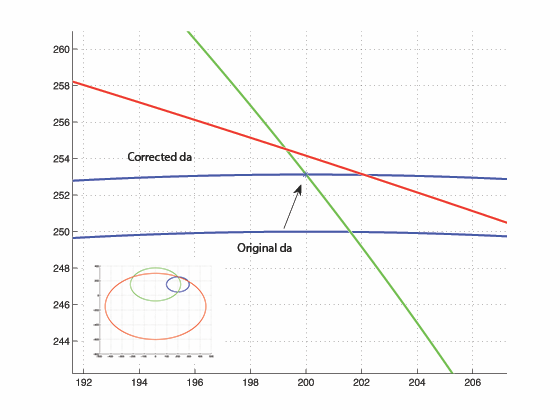
\includegraphics[scale=0.4]{p3.png}
\caption{Physical Meaning}
\medskip
\end{figure}

The combination of the $(x,y)$ means the location of the ship on condition accepting that there are certain amount of error within the $da$ which is calculated along with solving the nonlinear system.


In solving the actually problem, I used teacher's script called \textit{continuation.m} to give the problem a good initial guess and then I put generated initial guess into newton method and finally I used the line search method to increase the convergence area.

Because I noticed the 3 data was quite similar to the data in question a and I am confident with the convergence area of the method, I just used the answer from question a as the starting point which is $[201.0316,253.2789]$ and I assume the starting point for error e is 0.

\subsubsection{The results}
The generated answers are as follow:

\begin{center}
\begin{tabular}{ccccc}
& $x$&$y$&$e$\\ 
$q2b\_1$& $199.9756$& $253.1250$& $3.1250$\\
$q2b\_2$& $200.7137$& $255.8760$& $0.8775$\\
$q2b\_3$& $201.2004$& $253.4986$& $-0.0044$
\end{tabular}
\end{center}

There are two things worth noticing:
\begin{enumerate}
\item error $e$ can be negative that means the inital data for $da$ is too large.
\item as the quality of data improves, the error e itself decreases and the accuracy of $(x,y)$ is increasing.
\end{enumerate}

The releated convergence data:

\begin{verbatim}
q2b_1_convergence:
conpnewl(@q2b_1,@fdJacobian,[201.0316;253.2789;0],@continuation,@newtonSysL)
   t       |f(x)|
 0.00   976.095104
 0.03   943.553125
 0.07   911.011162
 0.10   878.469217
 0.13   845.927289
 0.17   813.385371
 0.20   780.843466
 0.23   748.301576
 0.27   715.759705
 0.30   683.217848
 0.33   650.676005
 0.37   618.134174
 0.40   585.592362
 0.43   553.050565
 0.47   520.508781
 0.50   487.967013
 0.53   455.425260
 0.57   422.883520
 0.60   390.341798
 0.63   357.800089
 0.67   325.258395
 0.70   292.716719
 0.73   260.175059
 0.77   227.633415
 0.80   195.091790
 0.83   162.550187
 0.87   130.008614
 0.90    97.467086
 0.93    64.925651
 0.97    32.384544
 1.00     0.292843

init_p =

  199.9757
  253.1250
    3.1264


 it    |f(x)|
 0     0.292843
     alpha    |f(x)|
     1.0000     0.000002
 1     0.000002
     alpha    |f(x)|
     1.0000     0.000000
 2     0.000000
 SUCCESS: Converged

ans =

  199.9756
  253.1250
    3.1250
    
q2b_2_convergence

conpnewl(@q2b_2,@fdJacobian,[201.0316;253.2789;0],@continuation,@newtonSysL)
   t       |f(x)|
 0.00   358.274081
 0.03   346.331062
 0.07   334.388042
 0.10   322.445019
 0.13   310.501998
 0.17   298.558978
 0.20   286.615956
 0.23   274.672937
 0.27   262.729916
 0.30   250.786898
 0.33   238.843880
 0.37   226.900861
 0.40   214.957840
 0.43   203.014820
 0.47   191.071799
 0.50   179.128779
 0.53   167.185759
 0.57   155.242736
 0.60   143.299712
 0.63   131.356692
 0.67   119.413672
 0.70   107.470646
 0.73    95.527628
 0.77    83.584606
 0.80    71.641587
 0.83    59.698567
 0.87    47.755546
 0.90    35.812525
 0.93    23.869505
 0.97    11.926491
 1.00     0.023922

init_p =

  200.7137
  253.8750
    0.8775


 it    |f(x)|
 0     0.023922
     alpha    |f(x)|
     1.0000     0.000000
 1     0.000000
 SUCCESS: Converged

ans =

  200.7137
  253.8750
    0.8775

q2b_3_convergence
conpnewl(@q2b_3,@fdJacobian,[201.0316;253.2789;0],@continuation,@newtonSysL)
   t       |f(x)|
 0.00   274.143177
 0.03   265.004945
 0.07   255.866713
 0.10   246.728481
 0.13   237.590250
 0.17   228.452017
 0.20   219.313785
 0.23   210.175552
 0.27   201.037318
 0.30   191.899086
 0.33   182.760855
 0.37   173.622622
 0.40   164.484390
 0.43   155.346157
 0.47   146.207926
 0.50   137.069695
 0.53   127.931464
 0.57   118.793231
 0.60   109.655000
 0.63   100.516768
 0.67    91.378536
 0.70    82.240304
 0.73    73.102072
 0.77    63.963840
 0.80    54.825610
 0.83    45.687377
 0.87    36.549146
 0.90    27.410914
 0.93    18.272682
 0.97     9.134451
 1.00     0.004433

init_p =

  201.2004
  253.4986
   -0.0044


 it    |f(x)|
 0     0.004433
     alpha    |f(x)|
     1.0000     0.000000
 1     0.000000
 SUCCESS: Converged

ans =

  201.2004
  253.4986
   -0.0044
\end{verbatim}

\section{Question 3}
Assuming U is in the format like ${[a1;a2;a3;a4;a5;v]}$.\\


Because I will use the above two in the coming questions, the expression written above was
actually working codes in the matlab files.
\subsection{Question a}
The F is the following:
\[
F=
\begin{bmatrix}
k*u(6)*\frac{u(1)}{G} + u(1) - a0\\
k*u(6)*\frac{u(2)}{G} + u(2) - u(1)\\
k*u(6)*\frac{u(3)}{G} + u(3) - u(2)\\
k*u(6)*\frac{u(4)}{G} + u(4) - u(3)\\
k*u(6)*\frac{u(5)}{G} + u(5) - u(4)\\
k*u(6)*a6/G + a6 - u(5)
\end{bmatrix}
\]

\subsection{Question b}
The Jacobian Matrix is the following:

\[
Jc
=
\begin{pmatrix}
1&0&0&0&0&k*\frac{u(1)}{G}\\
-1&1+k*\frac{u(6)}{G}&0&0&0&k*\frac{u(2)}{G}\\
0&-1&1+k*\frac{u(6)}{G}&0&0&k*\frac{u(3)}{G}\\
0&0&-1&1+k*\frac{u(6)}{G}&0&k*\frac{u(4)}{G}\\
0&0&0&-1&1+k*\frac{u(6)}{G}&k*\frac{u(5)}{G}\\
0&0&0&0&-1&k*\frac{a6}{G}
\end{pmatrix}
\]
\subsection{Question c}

In talking about the initial starting point I used the tutor's called \textit{continuation.m} to do a Homotopy Continuation assumption. And the stating point for solving the Homotopy continuation problem was a naive assumption, that $a6->a0$ is in decreasing order from 6 all the way down to 0 (and in here I assumed a5 to a1 as 5,4,3,2,1 respectively), and I picked up a random number 30 for the assumption of the size of V.

The solution is as following:
\[
x=
\begin{bmatrix}
4.1942\\
2.9318\\
2.0494\\
1.4326\\
1.0014\\
125.5833
\end{bmatrix}
\]

Which means a1 to a5 are equal to 4.1942 and 2.9318 and 2.0494 and 1.4326 and 1.0014 respectively and the size of v should be 125.5833). As we can see, $a6>a5>a4>a3>a2>a1$, so it is correct in terms of the decreasing order of the concentration.

\begin{enumerate}

\item The Matlab module for the evaluating function
\begin{verbatim} 
function eval = q3c(u)

% This is the function for the question 3

G = 35.0;
k = 0.12;
a0 = 6.0;
a6 = 0.7;

eval = [k*u(6)*u(1)/G + u(1) - a0;
    k*u(6)*u(2)/G + u(2) - u(1);
    k*u(6)*u(3)/G + u(3) - u(2);
    k*u(6)*u(4)/G + u(4) - u(3);
    k*u(6)*u(5)/G + u(5) - u(4);
    k*u(6)*a6/G + a6 - u(5)];
\end{verbatim}

\item The Matlab module for the Jacobian matrix:
\begin{verbatim}
function jc = cal_j(u)

% This is the jacobian matrix for question 3

G = 35.0;
k = 0.12;
a0 = 6.0;
a6 = 0.7;

jc = [1,0,0,0,0,k*u(1)/G;
    -1,1+k*u(6)/G,0,0,0,k*u(2)/G;
    0,-1,1+k*u(6)/G,0,0,k*u(3)/G;
    0,0,-1,1+k*u(6)/G,0,k*u(3)/G;
    0,0,0,-1,1+k*u(6)/G,k*u(5)/G;
    0,0,0,0,-1,k*a6/G];
\end{verbatim}

\item The solver:
\begin{verbatim}
% This script combining newton method and the homotopy continuation method.
% It use the homotopy continuation method to provide a good initial guess for the newton method.

% It was writeen to solve question 3

clear all
[init,less] = continuation(@q3c,@cal_j,[5;4;3;2;1;30],30);


[x,f] = newtonSys(@q3c,@cal_j,init,1e-4,30);
\end{verbatim}

\item The convergence data:
\begin{verbatim}
clear all
q3
   t       |f(x)|
 0.00     1.596292
 0.03     1.548111
 0.07     1.500060
 0.10     1.452148
 0.13     1.404380
 0.17     1.356766
 0.20     1.309315
 0.23     1.262038
 0.27     1.214945
 0.30     1.168052
 0.33     1.121374
 0.37     1.074930
 0.40     1.028741
 0.43     0.982833
 0.47     0.937236
 0.50     0.891985
 0.53     0.847125
 0.57     0.802707
 0.60     0.758796
 0.63     0.715470
 0.67     0.672829
 0.70     0.630994
 0.73     0.590121
 0.77     0.550408
 0.80     0.512106
 0.83     0.475538
 0.87     0.441117
 0.90     0.409365
 0.93     0.380931
 0.97     0.356589
 1.00     0.337208
 x     |f(x)|
 0     0.337208
 1     0.034869
 2     0.012595
 3     0.004078
 4     0.001468
 5     0.000518
 6     0.000184
 7     0.000065
 SUCCESS: Converged
\end{verbatim}

\end{enumerate}

\subsection{Question d}

Looking back at the question itself, it said that \textit{a series of n continuously-stirred reactor vessels, each of volume V}. So the physics meaning of the v is the size of the reactor vessels and as n=6 there are 6 of them and each of them is of the size of 125.5833. And the unit of the v can be conducted from the formula $\beta = \frac{k*v}{G}$. On condition that we knew beta and k and G's unit already.

\end{document}
